\documentclass[10pt]{article}
\usepackage[a4paper,margin=2.2cm]{geometry}
\usepackage[T1]{fontenc}
\usepackage[utf8]{inputenc}
\usepackage{lmodern}
\usepackage{microtype}
\usepackage{graphicx}
\usepackage{caption}
\usepackage{booktabs}
\usepackage{adjustbox}
\usepackage{array}
\usepackage{tabularx}
\usepackage{setspace}
\usepackage{enumitem}
\usepackage{multicol}
\usepackage[hidelinks]{hyperref}
\usepackage{url}
\captionsetup{font=small,labelfont=bf,justification=justified,singlelinecheck=false}
\setlength{\parindent}{0pt}
\setlength{\parskip}{0.55em}
\doublespacing
\setlist{itemsep=0.15em,topsep=0.3em,leftmargin=1.6em}
\emergencystretch=4em
\renewcommand{\thefigure}{S\arabic{figure}}
\renewcommand{\thetable}{S\arabic{table}}
\begin{document}

\begin{center}
{\Large\bfseries Additional file 1: Supporting Information\par}
\vspace{0.6em}
{\large\bfseries DMPNN Performance Estimates Diverge across Evaluation Boundaries in a Cyclic-Peptide Permeability Benchmark\par}
\vspace{0.8em}
Yutao Guo$^{1,2}$, Xujing Jiang$^{1,2}$, Zihan Zhang$^{1,2}$, Xuezhou Zhao$^{1,2}$, Mengxi Chen$^{1,2}$, Langzhe Zhang$^{1,2}$, Xiangyu Meng$^{1,2}$, Dan Wu$^{1,3,*}$\\
\vspace{0.35em}
\small $^{1}$International College of Pharmaceutical Innovation, Soochow University, Suzhou 215123, China\\
$^{2}$School of Pharmacy and Biomolecular Sciences, RCSI, 123 St Stephen's Green, Dublin 2, D02 VY51, Ireland\\
$^{3}$Department of Chemistry, RCSI, 123 St Stephen's Green, Dublin 2, D02 YN77, Ireland\\
$^{*}$Corresponding author: \href{mailto:danwu@suda.edu.cn}{danwu@suda.edu.cn}
\end{center}

\section*{Scope and analysis boundary}

This Supporting Information reports curation and split details, post-confirmatory robustness and sensitivity analyses for the frozen H1 comparison, a primary-source comparison with prior evaluation designs, the protocol timeline, deviations from the original split ladder, and the public-release inventory. Completed sensitivity analyses used the already accepted D0 out-of-fold predictions, checkpoint-only D3 residual reconstruction, or outcome-blind graph and curation inputs. No model was fitted, tuned, selected, replaced or recalibrated for those analyses. The internally prespecified 10,000-replicate block/seed bootstrap remains the inferential analysis for H1.

The H1 comparison used 6,895 curated records, 41 data sources, 18 frozen joint source/analogue blocks and five scheduled seeds. Joint-block and molecule-random prediction artifacts were verified against their frozen size and SHA-256 manifests before calculation.

The original version-2 split ladder listed molecule-grouped pseudorandom, chirality-aware Murcko, source-only, analogue-only and joint boundaries. Only the molecule-grouped and joint D0 arms were completed before outcome review. On 10 August 2026, source-only and analogue-only manifests were re-frozen operationally, and a newly added size-profile-matched molecule-random control was frozen, before any fit in those arms. Their pending results will be post-confirmatory and cannot alter the original H1 or H2 decisions. The Murcko arm remains uncompleted.

\section*{Curation accounting and fold assignment}

The raw PAMPA table contained 7,298 rows. A row was classified as irrecoverably censored when either source detection-limit field was populated; 372 rows met this frozen rule. The remaining 6,926 rows had parseable structures and sequences. They were grouped by source and isomeric canonical SMILES. Multi-row groups were collapsed only when year, database version, topology signature and canonical sequence agreed across uncensored rows; the analytical endpoint was their median. Exactly 31 compatible groups contained more than one eligible row, explaining the arithmetic difference between 6,926 usable raw rows and 6,895 curated records. There were no incompatible groups and no invalid structure/sequence rows in the frozen population.


\begin{table}[htbp]
\centering
\caption{Raw-to-curated accounting. The row-level curation manifest retains raw identifiers, censoring flags, inclusion or linked-exclusion status, and the final curated identifier.}
\begin{adjustbox}{max width=\textwidth}
\begin{tabular}{lrr}
\toprule
\textbf{Curation stage} & \textbf{Rows or groups} & \textbf{Rule} \\
\midrule
Raw PAMPA rows & 7,298 & Starting public table \\
Irrecoverably censored rows & 372 & Either detection-limit field populated \\
Uncensored usable rows & 6,926 & Parseable structure and sequence, numeric endpoint \\
Compatible multi-row groups collapsed & 31 & Same source and isomeric structure; compatible metadata; median endpoint \\
Curated source--structure records & 6,895 & Primary analytical population \\
Unique stereochemical molecules & 6,862 & \texttt{molecule\_\allowbreak{}id} assignment units \\
\bottomrule
\end{tabular}
\end{adjustbox}
\end{table}

For the molecule-grouped pseudorandom comparison, all records sharing \texttt{molecule\_\allowbreak{}id} remained in one fold. Molecule groups were sorted by decreasing size with stable structure-derived identifiers breaking ties, then placed into the currently smallest of five folds. Each fold contained 1,379 records. Complete sources and analogue components were allowed to cross this comparison boundary. In the joint analysis, neither a source nor an analogue component could cross the outer boundary.

\section*{H1 block influence and aggregation sensitivity}

Each frozen joint block was omitted in turn, and source-macro MAE was recalculated across the remaining sources for both evaluation arms. The difference was defined as joint-block MAE minus molecule-random MAE. This deletion analysis measures sensitivity to individual observed blocks; it does not define a new target population or confidence interval.

Alternative descriptive estimands assigned equal weight to records (row micro), sources (source macro) or blocks (block macro). For block-macro aggregation, source-specific MAEs were averaged within each block, blocks were weighted equally within each seed, and the five seed summaries were averaged.


\begin{table}[htbp]
\centering
\caption{H1 aggregation sensitivity. Values are means across five scheduled seeds. The three weighting schemes estimate different target quantities and are reported descriptively.}
\begin{adjustbox}{max width=\textwidth}
\begin{tabular}{lrrr}
\toprule
\textbf{Analysis} & \textbf{Joint-block MAE} & \textbf{Molecule-random MAE} & \textbf{Gap} \\
\midrule
Row micro & 0.6430 & 0.2928 & 0.3502 \\
Source macro & 1.0046 & 0.4672 & 0.5373 \\
Equal-block macro & 0.9048 & 0.4386 & 0.4662 \\
\bottomrule
\end{tabular}
\end{adjustbox}
\end{table}


\begin{figure}[htbp]
  \centering
  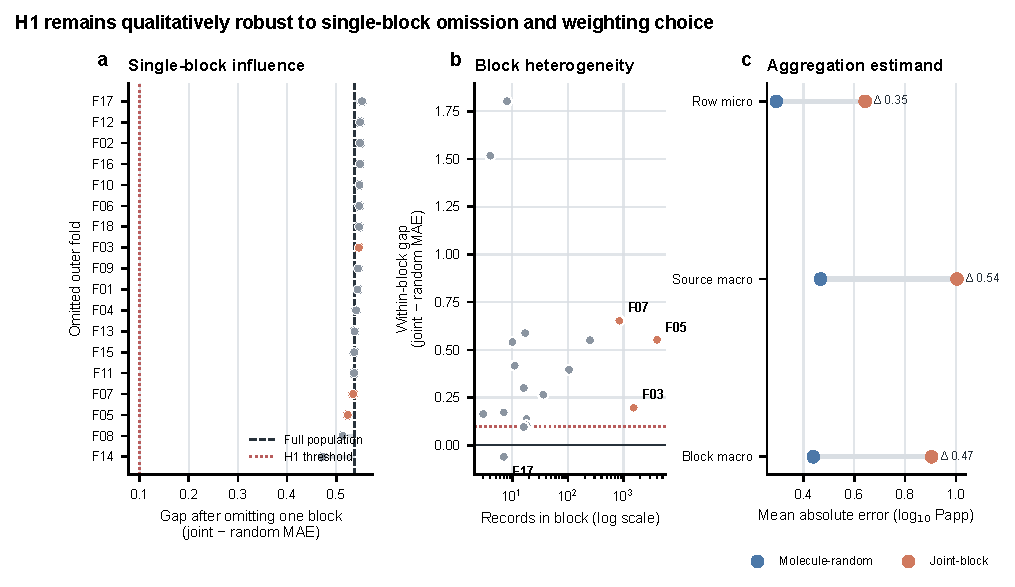
\includegraphics[width=0.98\textwidth]{figures/figure_s1_h1_block_influence.pdf}
  \caption{\textbf{H1 influence and aggregation sensitivity.} \textbf{a,} The D0 source-macro mean absolute error (MAE) gap between joint-block and molecule-random evaluation after omitting each of the 18 frozen joint blocks in turn. Points are ordered by the recalculated gap and labelled by the omitted outer fold. The black dashed line marks the full-population gap (0.537 log10 Papp units), and the red dotted line marks the preregistered 0.10 point-gap threshold. Orange points identify omission of one of the three largest blocks. \textbf{b,} Within-block source-macro gap versus frozen block record count for all 18 blocks. The three largest blocks and the sole block with a negative within-block gap are labelled. The x axis is logarithmic; the red dotted line marks a gap of 0.10. \textbf{c,} Five-seed mean D0 MAE under row-micro, source-macro and equal-block-macro aggregation. Blue and orange points denote molecule-random and joint-block evaluation, respectively, and connecting segments show the corresponding gap. All panels use the already frozen 6,895-record, 41-source prediction population across five scheduled seeds. These post-confirmatory analyses involved no refitting or model selection and are descriptive; the original block/seed bootstrap remains the inferential H1 analysis.}
  \label{fig:S1}
\end{figure}

\section*{Small-cluster and high-leverage sensitivity}

The five accepted seeds were first averaged within each source, giving 41 paired source-level joint-minus-random MAE differences nested in 18 sealed blocks. Three calculations then examined sensitivity to the small and unequal cluster set. An intercept-only CR1 variance estimator clustered the paired source differences by sealed block and used a t critical value with 17 degrees of freedom. A delete-one-block jackknife used the same t reference. Finally, all $2^{18}$ assignments obtained by independently changing the sign of each block contribution were enumerated.


\begin{table}[htbp]
\centering
\caption{Small-cluster sensitivity of the H1 source-macro gap. Delete-one-block point estimates ranged from 0.4724 to 0.5523. Seventeen of 18 block-specific mean gaps were positive, and 4 of 262,144 sign assignments were at least as extreme as observed. These analyses are post-confirmatory. CR1 and jackknife calculations treat the 18 blocks as independent clusters; the sign-flip test additionally assumes joint sign symmetry under the null. None replaces the internally prespecified block/seed bootstrap or creates additional independent regimes.}
\begin{adjustbox}{max width=\textwidth}
\begin{tabular}{lrrr}
\toprule
\textbf{Sensitivity} & \textbf{Estimate} & \textbf{Standard error} & \textbf{95\% interval or p value} \\
\midrule
CR1 block-clustered t interval & 0.5373 & 0.0757 & 0.3777--0.6970 \\
Delete-one-block jackknife t interval & 0.5373 & 0.0756 & 0.3779--0.6968 \\
Exhaustive block sign flip & 0.5373 & — & p = 0.00001526 \\
\bottomrule
\end{tabular}
\end{adjustbox}
\end{table}

\section*{Source-stratified error and point-prediction calibration}

Absolute and signed errors were summarized within each source and seed, then averaged across the five seeds. Positive signed error denotes predicted permeability that is too high (less negative log10 Papp), whereas negative signed error denotes predicted permeability that is too low. Sources were retained regardless of size; extreme estimates from small sources are localization diagnostics rather than stable independent effects.

For point-prediction calibration, the five OOF predictions for each record were averaged first. Records were divided into ten equal-frequency prediction bins separately within each evaluation arm. Mean observed permeability was compared with mean predicted permeability in each bin. Calibration slope was obtained from a descriptive least-squares regression of observed values on mean predictions; no recalibration function was fitted or applied.


\begin{table}[htbp]
\centering
\caption{Source-level bias and point-prediction calibration. Calibration used one five-seed mean OOF prediction per record. Prediction bins were arm-specific and contained all 6,895 records.}
\begin{adjustbox}{max width=\textwidth}
\begin{tabular}{lrr}
\toprule
\textbf{Calibration summary} & \textbf{Joint-block} & \textbf{Molecule-random} \\
\midrule
Calibration slope & 0.5950 & 0.9637 \\
Calibration intercept & -2.2192 & -0.2075 \\
Pearson correlation & 0.3252 & 0.8729 \\
Global signed bias & -0.1746 & -0.0010 \\
Decile-weighted absolute calibration error & 0.1808 & 0.0269 \\
Median absolute source bias & 0.5779 & 0.0784 \\
Sources with absolute bias above 0.5 & 23 of 41 & 3 of 41 \\
\bottomrule
\end{tabular}
\end{adjustbox}
\end{table}


\begin{figure}[htbp]
  \centering
  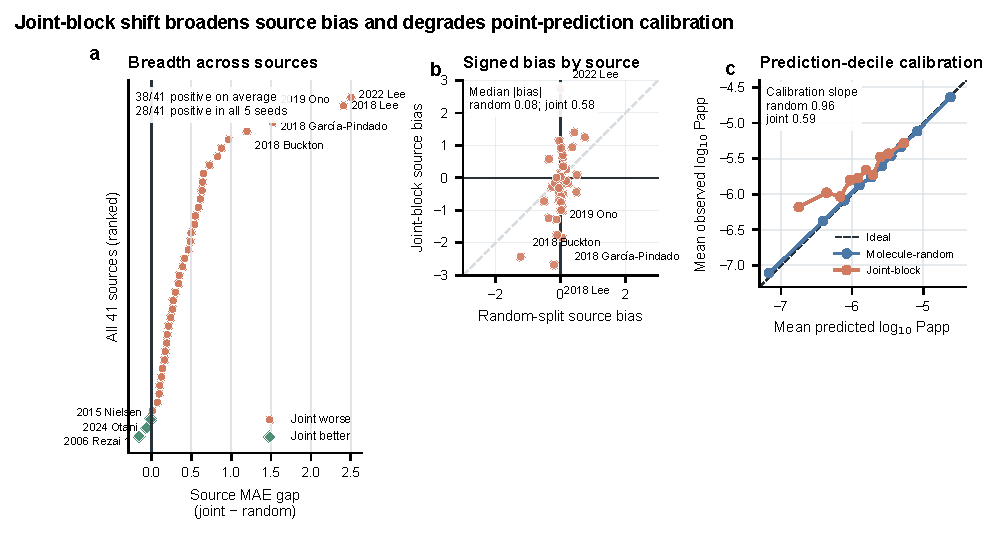
\includegraphics[width=0.98\textwidth]{figures/figure_s2_h1_stratified_calibration.pdf}
  \caption{\textbf{Source-stratified error and point-prediction calibration.} \textbf{a,} Ranked source-level D0 MAE difference between joint-block and molecule-random evaluation for all 41 frozen sources. Orange circles indicate a higher joint-block MAE and green diamonds indicate a lower joint-block MAE; labelled points are the five largest positive differences and all three negative differences. Source summaries are means across five scheduled seeds. \textbf{b,} Five-seed mean signed error for each source under molecule-random and joint-block evaluation. Positive values indicate predicted permeability that is too high and negative values indicate predicted permeability that is too low. The dashed diagonal indicates equal bias under the two evaluation schemes; the five largest absolute joint-block biases are labelled. \textbf{c,} Point-prediction calibration after averaging the five frozen OOF predictions for each of 6,895 records. Points show mean observed versus mean predicted log10 Papp within ten equal-frequency, arm-specific prediction bins; the dashed diagonal is ideal calibration. Slopes are from descriptive least-squares regressions of observed on mean predicted values. No refitting, recalibration or model selection was performed. Source data are provided as CSV files.}
  \label{fig:S2}
\end{figure}

\section*{Analogue-threshold sensitivity of evidence geometry}

The outcome-blind analogue graph was reconstructed at the prespecified descriptive chiral ECFP4 Tanimoto thresholds of 0.70, 0.80 and 0.90. Fingerprint radius and length, chirality, the molecular-weight-ratio constraint, the exact one-token cyclic-edit relation, source provenance and all public curated records were held fixed. The threshold-0.80 reconstruction exactly reproduced every frozen primary component and block identifier.

Alternative thresholds were used only to compare graph and partition geometry. Existing OOF predictions were not rescored under these partitions because their training/test boundaries differ. A valid alternative-threshold performance comparison would require complete newly frozen nested retraining and would be exploratory after release of the primary outcomes.


\begin{table}[htbp]
\centering
\caption{Outcome-blind analogue-threshold sensitivity. The effective block count is the inverse Simpson concentration index calculated from record shares.}
\begin{adjustbox}{max width=\textwidth}
\begin{tabular}{lrrrrrr}
\toprule
\textbf{Tanimoto threshold} & \textbf{Analogue edges} & \textbf{Analogue components} & \textbf{Joint blocks} & \textbf{Largest block share} & \textbf{Top-three share} & \textbf{Effective blocks} \\
\midrule
0.70 & 648,106 & 91 & 15 & 58.80\% & 93.02\% & 2.435 \\
0.80 & 141,425 & 305 & 18 & 58.16\% & 92.39\% & 2.480 \\
0.90 & 38,787 & 745 & 20 & 57.84\% & 92.07\% & 2.504 \\
\bottomrule
\end{tabular}
\end{adjustbox}
\end{table}


\begin{figure}[htbp]
  \centering
  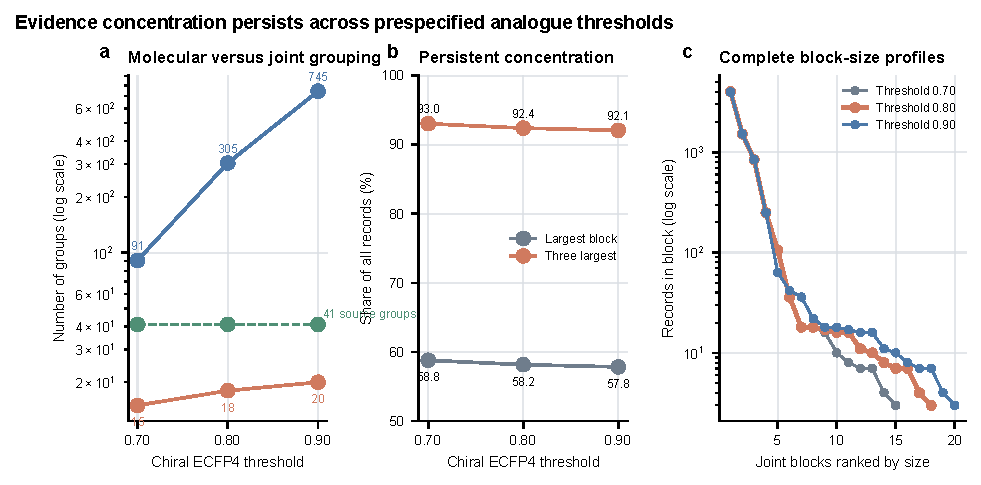
\includegraphics[width=0.98\textwidth]{figures/figure_s3_block_definition_sensitivity.pdf}
  \caption{\textbf{Analogue-threshold sensitivity of evidence geometry.} \textbf{a,} Number of analogue components (blue) and source/component joint blocks (orange) reconstructed at chiral ECFP4 Tanimoto thresholds of 0.70, 0.80 and 0.90; the 41 source groups are shown as a green dashed reference. Counts use a logarithmic axis. The molecular-weight-ratio constraint, exact one-token cyclic-edit rule and source closure were held fixed. \textbf{b,} Percentage of all 6,895 records contained in the largest and three largest joint blocks at each threshold. \textbf{c,} Complete ranked joint-block size distributions on a logarithmic axis. The frozen primary threshold of 0.80 is emphasized in orange. Reconstruction used only public structure and provenance fields and exactly reproduced every primary 0.80 component/block identifier. No outcome, prediction or model-performance value was used. Alternative thresholds describe partition geometry only and were not used to rescore the frozen OOF predictions. Source data are provided as CSV files.}
  \label{fig:S3}
\end{figure}

\section*{Prior-work comparison of evaluation boundaries}

The comparison below was updated from primary reports through 10 August 2026. It is intended to delimit the present contribution, not to claim novelty for source holdout, chemical clustering, scaffold splitting, nested validation, or similarity-aware splitting individually.


\begin{table}[htbp]
\centering
\caption{Primary-source comparison of evaluation boundaries. Geylan et al. is the closest provenance-aware precedent located. The present distinction is simultaneous closure of alternating source--analogue paths throughout model development. This is a search-limited comparison, not proof that no unindexed or unpublished study used a similar design. A post-confirmatory source-only, analogue-only and size-profile-matched random ladder has been frozen but is not yet reported.}
\scriptsize
\setlength{\tabcolsep}{3pt}
\renewcommand{\arraystretch}{1.15}
\begin{tabularx}{\textwidth}{>{\raggedright\arraybackslash}p{0.13\textwidth}>{\raggedright\arraybackslash}X>{\centering\arraybackslash}p{0.105\textwidth}>{\centering\arraybackslash}p{0.12\textwidth}>{\raggedright\arraybackslash}p{0.19\textwidth}}
\toprule
\textbf{Study} & \textbf{Reported evaluation boundary} & \textbf{Complete source held out?} & \textbf{Transitive analogue component held out?} & \textbf{Same boundary throughout nested development?} \\
\midrule
Geylan et al. (2024) & Four large external sources; separate source-group and canonical-group scenarios & Yes, in source arms & No & Partly; grouping scenarios were separate \\
CycPeptMP (2024) & Kennard--Stone holdout plus cross-validation & No & No & No \\
PeptideCLM (2025) & Six embedding/PCA clusters, leave one cluster out & No & No & Development within retained clusters, not joint blocks \\
MultiCycPermea (2025) & Random, Murcko/Jaccard-cluster OOD and permeability-cliff settings & No & No & No joint source--analogue nesting \\
13-method benchmark (2025) & Random and Murcko-scaffold splits; external set & No & No & No joint source--analogue nesting \\
DataSAIL (2025) & Generic similarity-aware one- and two-dimensional constrained splits & User-defined & User-defined & Depends on the user workflow \\
Present study & Molecule-grouped pseudorandom and joint source--analogue connected-component LOBO & Yes & Yes & Yes for the accepted joint analysis \\
\bottomrule
\end{tabularx}
\end{table}

Primary report identifiers: Geylan et al., DOI 10.1039/D4DD00056K; CycPeptMP, DOI 10.1093/bib/bbae417; PeptideCLM, DOI 10.1021/acs.jcim.4c01441; MultiCycPermea, DOI 10.1186/s12915-025-02166-2; 13-method benchmark, DOI 10.1186/s13321-025-01083-4; DataSAIL, DOI 10.1038/s41467-025-58606-8.

\section*{Protocol timeline and public identifiers}


\begin{table}[htbp]
\centering
\caption{Protocol and release timeline. The complete chronology, file hashes and distinction between an internal freeze and an independently time-stamped public preregistration are provided in \texttt{PUBLIC\_\allowbreak{}PROTOCOL\_\allowbreak{}TIMELINE.md}. The public repository is \url{https://github.com/schwarzeteeguo-creator/scaffoldseal-cp-evaluation} and the archived release is \url{https://doi.org/10.5281/zenodo.22126300.} Local hashes alone are not described as independent public preregistration.}
\scriptsize
\setlength{\tabcolsep}{3pt}
\renewcommand{\arraystretch}{1.15}
\begin{tabularx}{\textwidth}{>{\raggedright\arraybackslash}p{0.13\textwidth}>{\raggedright\arraybackslash}X>{\raggedright\arraybackslash}p{0.31\textwidth}}
\toprule
\textbf{Date} & \textbf{Protocol event} & \textbf{Public-release evidence} \\
\midrule
2026-07-17 & Original v1 feasibility gate failed; compromised v1 final partition and vault retired & Failed protocol, decisions D-018/D-019 and repair audit retained \\
2026-07-17 & Version-2 recovery map, CV governance and experiment plan frozen internally before any v2 fit & File hashes listed in \texttt{PUBLIC\_\allowbreak{}PROTOCOL\_\allowbreak{}TIMELINE.md}; no independent public timestamp \\
2026-07-17 to 2026-07-19 & Pre-fit split, preprocessing, stopping and prediction controls reviewed & Test and audit records; training remained blocked until acceptance \\
2026-07-26 to 2026-07-27 & H1 random-comparison plan accepted and executed & Accepted stage manifests, sealed OOF predictions and bootstrap outputs \\
2026-08-09 & D123 sealed audit and one controlled metric release & Decisions D-052 to D-054 and H2 verdict report \\
2026-08-10 & Zero-training sensitivity analyses and split-boundary completion plan frozen & Reporting scripts, input hashes and post-confirmatory internal freeze \\
\bottomrule
\end{tabularx}
\end{table}

\section*{Itemized Supporting Information and release mapping}


\begin{table}[htbp]
\centering
\caption{Mapping of SI statements to actual files. The authoritative package-level checklist is \texttt{RELEASE\_\allowbreak{}INVENTORY\_\allowbreak{}V0.7.md}. A manuscript statement must be removed or marked pending if its corresponding released file is absent.}
\scriptsize
\setlength{\tabcolsep}{3pt}
\renewcommand{\arraystretch}{1.15}
\begin{tabularx}{\textwidth}{>{\raggedright\arraybackslash}p{0.19\textwidth}>{\raggedright\arraybackslash}X>{\raggedright\arraybackslash}p{0.25\textwidth}}
\toprule
\textbf{SI item} & \textbf{Local/release files} & \textbf{Status in this version} \\
\midrule
Curation accounting & \texttt{curation\_\allowbreak{}manifest\_\allowbreak{}release\_\allowbreak{}safe.csv}; \texttt{curated\_\allowbreak{}group\_\allowbreak{}manifest\_\allowbreak{}release\_\allowbreak{}safe.csv}; audit JSON; curation code and hashes & Included as release-safe manifests; structures and endpoint labels excluded \\
Primary joint split & outer record assignments, outer-fold manifest and inner-basket manifest & Complete and frozen \\
Comparison splits & molecule-grouped assignments; source-only, analogue-only and matched-size manifests & Outcome-blind manifests complete; corresponding model results pending \\
H1 headline & accepted joint/random metric files, OOF manifests and bootstrap output & Complete and frozen \\
H1 influence and aggregation & \texttt{analyze\_\allowbreak{}h1\_\allowbreak{}block\_\allowbreak{}influence.py}; three CSVs; JSON summary; Fig. S1 & Complete \\
H1 source calibration & \texttt{analyze\_\allowbreak{}h1\_\allowbreak{}stratified\_\allowbreak{}calibration.py}; four CSVs; JSON summary; Fig. S2 & Complete \\
Analogue-threshold geometry & \texttt{analyze\_\allowbreak{}block\_\allowbreak{}definition\_\allowbreak{}sensitivity.py}; four CSVs; JSON summary; Fig. S3 & Complete \\
H1 small-cluster sensitivity & \texttt{analyze\_\allowbreak{}h1\_\allowbreak{}small\_\allowbreak{}cluster\_\allowbreak{}sensitivity.py}; paired-source, cluster, deletion CSVs; JSON summary & Complete \\
Censoring and source metadata & \texttt{analyze\_\allowbreak{}curation\_\allowbreak{}source\_\allowbreak{}audit.py}; release-safe manifests; source and note summaries; JSON & Complete; no raw structures or labels redistributed \\
D3 coverage aggregation & \texttt{analyze\_\allowbreak{}d3\_\allowbreak{}coverage\_\allowbreak{}stratification.py}; per-seed, per-fold and per-source CSVs; JSON & Complete; checkpoint-only predictions, no fitting \\
Prior-work boundary comparison & \texttt{PRIOR\_\allowbreak{}WORK\_\allowbreak{}COMPARISON\_\allowbreak{}NOTES.md}; \texttt{prior\_\allowbreak{}work\_\allowbreak{}evaluation\_\allowbreak{}comparison.csv} & Complete through search date \\
Protocol and frozen files & v2 internal protocol, research map, CV governance, experiment plan, deviation table and public timeline & Complete locally; external timestamp absent \\
Public archive metadata & release checksum, \texttt{CITATION.cff}, license, GitHub URL and Zenodo DOI & Archived at \url{https://doi.org/10.5281/zenodo.22126300} \\
\bottomrule
\end{tabularx}
\end{table}

\section*{Censoring and source-metadata audit}

The frozen curation rule excluded every row for which either detection-limit field was populated. A zero-training audit classified the two free-text fields conservatively and checked whether an excluded source-structure group was otherwise represented by an uncensored replicate. The classes below describe database annotations; they are not assumed to be mutually commensurate assay bounds.


\begin{table}[htbp]
\centering
\caption{Censoring semantics and retained-group linkage. Note classes sum to 372. Numeric database entries among the excluded rows were heterogeneous: 270 were recorded as -10, 45 as -7, 15 as -4, and the remainder used other values. The raw table provided no harmonized structured columns for PAMPA pH, membrane composition, incubation time, temperature, or donor/acceptor conditions. Accordingly, the analysis neither substituted sentinel values as ordinary endpoints nor imposed a universal quantitative censoring bound. Source identity is treated as a combined provenance and protocol proxy.}
\scriptsize
\setlength{\tabcolsep}{3pt}
\renewcommand{\arraystretch}{1.15}
\begin{tabularx}{\textwidth}{>{\raggedright\arraybackslash}X>{\centering\arraybackslash}p{0.22\textwidth}}
\toprule
\textbf{Audit item} & \textbf{Rows or sources} \\
\midrule
Excluded rows carrying a detection-limit annotation & 372 \\
Raw-data sources containing at least one excluded row & 23 \\
Database-assigned or reported floor & 259 \\
Explicit upper limit & 40 \\
No reportable value & 19 \\
Not detected or below limit of detection & 9 \\
Solubility failure or not tested & 7 \\
Other detection-limit note & 38 \\
Excluded rows linked to a retained uncensored group & 2 \\
Excluded rows without a retained continuous-endpoint group & 370 \\
Completely censored source & 1 source, 10 rows \\
\bottomrule
\end{tabularx}
\end{table}

\section*{Protocol completion and deviations}


\begin{table}[htbp]
\centering
\caption{Completion and evidential status of planned and added analyses. Source-only and analogue-only boundaries were listed in the original plan but were not completed before the joint and molecule-grouped outcomes were opened. Their operational re-freeze does not restore confirmatory status. The matched-size control was added only after recognizing that the completed H1 comparison changed both dependence and training-size profiles.}
\scriptsize
\setlength{\tabcolsep}{3pt}
\renewcommand{\arraystretch}{1.15}
\begin{tabularx}{\textwidth}{>{\raggedright\arraybackslash}p{0.18\textwidth}>{\raggedright\arraybackslash}p{0.22\textwidth}>{\raggedright\arraybackslash}p{0.24\textwidth}>{\raggedright\arraybackslash}X}
\toprule
\textbf{Planned element} & \textbf{Status before outcome review} & \textbf{Status in this version} & \textbf{Evidential role} \\
\midrule
Joint source/analogue D0 & Completed & Reported & Primary internally prespecified evaluation \\
Molecule-grouped pseudorandom D0 & Completed & Reported & Internally prespecified H1 comparison \\
Chirality-aware Murcko D0 & Not completed & Pending & Originally planned secondary boundary; no result implied \\
Source-only D0 & Not completed & Outcome-blind manifest re-frozen 10 August & Post-confirmatory when run \\
Analogue-only D0 & Not completed & Outcome-blind manifest re-frozen 10 August & Post-confirmatory when run \\
Size-profile-matched molecule-random D0 & Not in original ladder & Newly frozen 10 August; pending & Post-confirmatory training-size control \\
D1-D3 joint-block ladder & Completed & Reported & Internally prespecified H2 tests and ablations \\
Prospective matched-assay H3 & Not performed & Pending external data & Future prospective confirmation \\
\bottomrule
\end{tabularx}
\end{table}

\section*{D3 coverage aggregation sensitivity}

Each curated record contributed five algorithmic seed realizations to the primary slot-pooled coverage denominator. These realizations are useful for measuring execution variability but are not independent experimental observations. We therefore report the seed range and equal-source and equal-block descriptive estimands without a binomial confidence interval.


\begin{table}[htbp]
\centering
\caption{Sensitivity of D3 empirical-interval coverage to aggregation. Slot pooling weights every record-seed pair equally; source and block macro estimates weight the 41 sources and 18 outer blocks equally, respectively. The wide block range reflects highly unequal and sometimes very small omitted regimes. All aggregations show under-coverage at the higher nominal levels.}
\scriptsize
\setlength{\tabcolsep}{3pt}
\renewcommand{\arraystretch}{1.15}
\begin{tabularx}{\textwidth}{>{\centering\arraybackslash}p{0.12\textwidth}>{\centering\arraybackslash}p{0.11\textwidth}>{\centering\arraybackslash}p{0.17\textwidth}>{\centering\arraybackslash}p{0.15\textwidth}>{\centering\arraybackslash}p{0.14\textwidth}>{\centering\arraybackslash}X}
\toprule
\textbf{Nominal coverage} & \textbf{Slot-pooled} & \textbf{Per-seed range} & \textbf{Equal-source macro} & \textbf{Equal-block macro} & \textbf{Block range} \\
\midrule
50\% & 44.1\% & 41.9-46.9\% & 31.9\% & 28.4\% & 0.0-80.0\% \\
80\% & 67.2\% & 65.4-68.7\% & 58.6\% & 59.5\% & 0.0-100.0\% \\
90\% & 77.0\% & 75.8-78.1\% & 71.4\% & 75.0\% & 0.0-100.0\% \\
\bottomrule
\end{tabularx}
\end{table}

\section*{Source-data files}

The influence package contains \texttt{h1\_\allowbreak{}leave\_\allowbreak{}one\_\allowbreak{}block\_\allowbreak{}out.csv}, \texttt{h1\_\allowbreak{}aggregation\_\allowbreak{}sensitivity.csv} and \texttt{h1\_\allowbreak{}per\_\allowbreak{}block\_\allowbreak{}effect.csv}.

The stratified-calibration package contains \texttt{h1\_\allowbreak{}source\_\allowbreak{}stratified\_\allowbreak{}metrics.csv}, \texttt{h1\_\allowbreak{}block\_\allowbreak{}stratified\_\allowbreak{}metrics.csv}, \texttt{h1\_\allowbreak{}prediction\_\allowbreak{}decile\_\allowbreak{}calibration.csv} and \texttt{h1\_\allowbreak{}calibration\_\allowbreak{}summary.csv}.

The threshold-sensitivity package contains \texttt{block\_\allowbreak{}definition\_\allowbreak{}threshold\_\allowbreak{}summary.csv}, \texttt{block\_\allowbreak{}definition\_\allowbreak{}ranked\_\allowbreak{}sizes.csv}, \texttt{block\_\allowbreak{}definition\_\allowbreak{}partition\_\allowbreak{}comparison.csv} and \texttt{block\_\allowbreak{}definition\_\allowbreak{}record\_\allowbreak{}assignments.csv}.

The small-cluster package contains \texttt{h1\_\allowbreak{}paired\_\allowbreak{}source\_\allowbreak{}effects.csv}, \texttt{h1\_\allowbreak{}cluster\_\allowbreak{}contributions.csv}, \texttt{h1\_\allowbreak{}small\_\allowbreak{}cluster\_\allowbreak{}delete\_\allowbreak{}one.csv} and \texttt{h1\_\allowbreak{}small\_\allowbreak{}cluster\_\allowbreak{}sensitivity\_\allowbreak{}summary.json}.

The literature package contains \texttt{prior\_\allowbreak{}work\_\allowbreak{}evaluation\_\allowbreak{}comparison.csv} and \texttt{PRIOR\_\allowbreak{}WORK\_\allowbreak{}COMPARISON\_\allowbreak{}NOTES.md}.

The curation/source-audit package contains \texttt{source\_\allowbreak{}censoring\_\allowbreak{}and\_\allowbreak{}endpoint\_\allowbreak{}summary.csv}, \texttt{censoring\_\allowbreak{}note\_\allowbreak{}class\_\allowbreak{}summary.csv}, \texttt{censored\_\allowbreak{}database\_\allowbreak{}numeric\_\allowbreak{}values.csv}, \texttt{curation\_\allowbreak{}manifest\_\allowbreak{}release\_\allowbreak{}safe.csv}, \texttt{curated\_\allowbreak{}group\_\allowbreak{}manifest\_\allowbreak{}release\_\allowbreak{}safe.csv}, \texttt{curation\_\allowbreak{}source\_\allowbreak{}audit\_\allowbreak{}summary.json} and \texttt{SHA256SUMS}.

The D3 coverage-stratification package contains \texttt{d3\_\allowbreak{}coverage\_\allowbreak{}by\_\allowbreak{}seed.csv}, \texttt{d3\_\allowbreak{}coverage\_\allowbreak{}by\_\allowbreak{}outer\_\allowbreak{}fold.csv}, \texttt{d3\_\allowbreak{}coverage\_\allowbreak{}by\_\allowbreak{}source.csv}, \texttt{d3\_\allowbreak{}coverage\_\allowbreak{}aggregation\_\allowbreak{}sensitivity.csv}, \texttt{d3\_\allowbreak{}coverage\_\allowbreak{}stratification\_\allowbreak{}summary.json} and \texttt{SHA256SUMS}.


\end{document}
